\documentclass[twoside,10pt]{article}
\usepackage{/Users/bradenhoagland/latex/styles/toggles}
%\toggletrue{sectionbreaks}
%\toggletrue{sectionheaders}
\newcommand{\docTitle}{Math 323 - HW 9}
\usepackage{/Users/bradenhoagland/latex/styles/common}
\importStyles{modern}{rainbow}{boxy}

%\renewcommand{\theenumi}{\alph{enumi}}

\begin{document}
%\tableofcontents

% ------------------------------
% 6.17
% ------------------------------
\begin{exer}[6.17]
If alternate interior angles of a transversal $\ell$ to two lines $\ell_1$ and $\ell_2$ are equal, then $\ell_1$ and $\ell_2$ are ultraparallel.
\end{exer}

We must show that $\ell_1$ and $\ell_2$ do not intersect and are not parallel.

\textbf{Do not intersect:} Suppose $\ell_1$ and $\ell_2$ intersect at a point $C$, and suppose $\ell$ crosses $\ell_1$ and $\ell_2$ at points $A$ and $B$, respectively.

\begin{figure}[H]
	\centering
	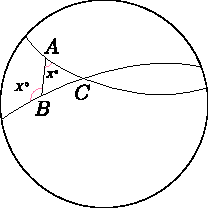
\includegraphics[scale=1.5]{fig/17a.pdf}
	%\caption{}
\end{figure}

Then $\Delta ABC$ is a bounded triangle, so by Theorem 6.10, its angles sum to strictly less than $180\degree$. But if the alternate interior angles of $\ell$ are both $X\degree$, then the sum of the angles of $\Delta ABC$ is greater than or equal to
\[
X\degree + 180\degree - X\degree \geq 180\degree .
\] Thus by contradiction, $\ell_1$ and $\ell_2$ do not intersect.

\textbf{Not parallel:} If $\ell_1$ and $\ell_2$ are parallel, then the alternate interior angles of $\ell$ are all $\pi/2$, which means $\beta=\pi/2$.

\begin{figure}[H]
	\centering
	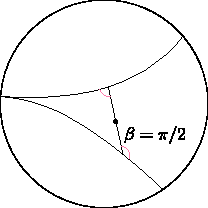
\includegraphics[scale=1.5]{fig/17b.pdf}
	%\caption{}
\end{figure}

But $\beta=\pi/2$ contradicts the fifth axiom of hyperbolic geometry from the textbook, so $\ell_1$ and $\ell_2$ cannot be parallel.

\newpage

% ------------------------------
% 6.18
% ------------------------------
\begin{exer}[6.18]
Two parallel lines do not have a common perpendicular. Where does the proof of Theorem 6.15 fail in this case? That is, where was it important that the two lines in Theorem 6.15 be ultraparallel?
\end{exer}

If the two lines are perpendicular, then $\beta \to 0$ instead of being bound below by $\Pi(|PQ|)$. This makes the constructed transversal from the proof have angle 0 with both lines, which is a contradiction since the two lines never intersect.

\newpage

% ------------------------------
% 6.23
% ------------------------------
\begin{exer}[6.23]
Any two triply asymptotic triangles are congruent.
\end{exer}

All three lines composing a triply asymptotic triangle intersect at infinity and are thus parallel. This means all three angles in the triangle are 0. Since this is true for any triply asymptotic triangle, they are all similar. Then by Theorem 6.22 (since triply asymptotic triangles are certainly also doubly asymptotic), any two triply asymptotic triangles are congruent.

\newpage

% ------------------------------
% 6.25
% ------------------------------
\begin{exer}[6.25]
	The area of a doubly asymptotic triangle is finite.
\end{exer}

Suppose $\Delta ABC$ is doubly asymptotic with $B,C$ at infinity. If $D$ is a finite point on $BC$, then $|\Delta ABC| = |\Delta ABD| + |\Delta ACD|$, as shown below.

\begin{figure}[H]
	\centering
	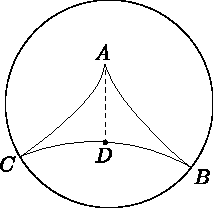
\includegraphics[scale=1.5]{fig/25.pdf}
	%\caption{}
\end{figure}

But $\Delta ABD$ and $\Delta ACD$ are both singly asymptotic triangles, so by Theorem 6.24, both have finite area. Then since the finite sum of finite values is finite, $|\Delta ABC|$ is finite.

\newpage

% ------------------------------
% 10.2
% ------------------------------
\begin{exer}[10.2]
What is the area of a quadrialteral $ABCD$ in the sphere? A polygon?
\end{exer}

We'll do this just for general polygons, as the quadrilateral is a special case. We'll prove that the area of an $n$-gon $X_1 \dots X_n$ on the sphere is
\[
	\rho^2 (X_1 + \dots + X_n - n\pi),
\] where $\rho$ is the radius of the sphere. To show this by induction, note that our base case is just Theorem 10.1 ($n=1$). Suppose that this holds for $(n-1)$-gons, then we want to show it for $n$-gons.

Let $X_1 \dots X_n$ be some $n$-gon, then we can decompose it into an $(n-1)$-gon $X_1 \dots X_{n-1}$ and a triangle $X_{n-1}X_{n}X_1$, as shown below.

\begin{figure}[H]
	\centering
	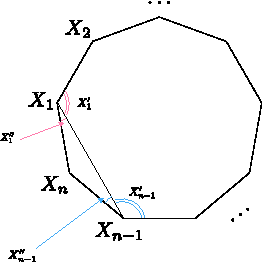
\includegraphics[scale=1.4]{fig/2.pdf}
	%\caption{}
\end{figure}

Then by our inductive hypothesis, the area of our $n$-gon is
\begin{align*}
	|X_1 \dots X_n| &= \rho^2\big(X_1'+ X_2 + X_3 + \dots + X_{n-2}+X_{n-1}' - (n-1)\pi \big) \\
			& \quad + \rho^2 \big( X_1'' + X_{n-1}'' + X_n - \pi\big) \\
			&= \rho^2 (X_1 + \dots + X_n - n \pi)
\end{align*}
since $X_1' + X_1'' + X_1$ and $X_{n-1}'+X_{n-1}'' = X_{n-1}$.

\newpage

% ------------------------------
% 10.3
% ------------------------------
\begin{exer}[10.3]
Show that the area of a circl of radius $r$ on a sphere of radius $\rho$ is
\[
	A = 4\pi\rho^2 \sin^2\left( \frac{r}{2\rho}  \right).
\] 
\end{exer}

Consider an arc from the center of the circle to a point on its outer edge. This has length $r$and is subtended by some angle $\phi_f$ at the center of the sphere, as shown below.

\begin{figure}[H]
	\centering
	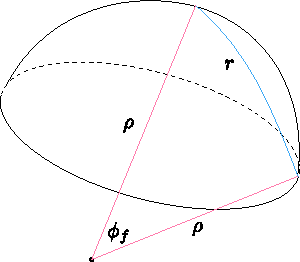
\includegraphics[scale=1.2]{fig/3.pdf}
	%\caption{}
\end{figure}

Since $r = \phi_f \rho$, we have $\phi_f = r/\rho$. Now to find the area of this surface, we can simply integrate over it using spherical coordinates:
\begin{align*}
	A &= \int_{0}^{2\pi} \int_{0}^{\phi_f} \rho^2 \sin \phi \;d\phi \;d\theta \\
	  &= 2\pi \rho^2 \int_{0}^{r/\rho} sin \phi \;d\phi \\
	  &= 2\pi \rho^2 \Big[ -\cos \phi \Big]_{0}^{r/\rho} \\
	  &= 2\pi \rho^2 \left( 1 - \cos\left( \frac{r}{\rho}  \right) \right).
	  \intertext{Then using the trig identity $\sin^2(\theta) = (1-\cos(2\theta))/2$, this becomes}
	  &= 4\pi\rho^2 \sin^2\left( \frac{r}{2\rho}  \right).
\end{align*}

\newpage

% ------------------------------
% 10.8
% ------------------------------
\begin{exer}[10.8]
Let $\Delta ABC$ be a right triangle on the unit sphere with right angle at $C$. Prove that
\[
\cos A = \cos a \sin B.
\] What is the corresponding result in Euclidean geometry.
\end{exer}

By Theorem 10.7,
\[
\sin B = \frac{\sin b}{\sin c} .
\] Then by this result and Theorem 10.7 again,
\[
\cos A = \frac{\cos a \sin b}{\sin c} = \cos a \sin B.
\] In Euclidean geometry,
\[
	B = \pi - \left( \frac{\pi}{2} +A \right) = \frac{\pi}{2} -A
\] and $\cos a = \cos 0 =1$, so this reduces to
\[
	\cos A = \sin\left( \frac{\pi}{2} -A \right).
\] 

\end{document}
